\documentclass[11pt]{article}
\usepackage{amsmath, amssymb, amsthm}
\usepackage[retainorgcmds]{IEEEtrantools}

\usepackage[pdftex]{graphicx}
\usepackage{tikz}
\usepackage{circuitikz}
\usetikzlibrary{intersections,decorations.pathmorphing}

\usepackage{fancyhdr}

%Listings stuff
\usepackage{listings}
\usepackage{lstautogobble}
\usepackage{color}

\definecolor{gray}{rgb}{0.5,0.5,0.5}
\lstset{
basicstyle={\small\ttfamily},
tabsize=3,
numbers=left,
numbersep=5pt,
numberstyle=\tiny\color{gray},
stepnumber=2,
breaklines=true,
boxpos=t
}

%Format stuff
\pagestyle{fancy}
\headheight 35pt

%Header info
\chead{\Large \textbf{Coupled Oscillators}}
\lhead{}
\rhead{}

\begin{document}
\section{Equal-Mass 2-Oscillator System}
Consider a simple example with two identical SHO's connected by a spring.

\begin{center}
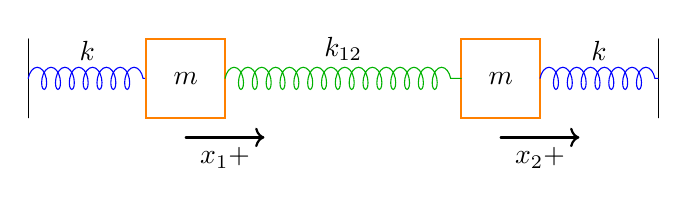
\begin{tikzpicture}
	[scale=1,line cap=round,
	%Styles
	axes/.style=,
	important line/.style={very thick},
	information text/.style={rounded corners,fill=red!10,inner sep=1ex},
	dot/.style={circle,inner sep=1pt,fill,label={#1},name=#1},
	spring/.style={decorate,decoration={coil,amplitude=4pt, segment length=5pt}}			
	]
	
	%Colors
	\colorlet{anglecolor}{green!50!black}	%angle arcs/lines
	
	%The graphic
	\draw (0,0) -- (0,1);
	\draw (8,0) -- (8,1);
	
	\draw[spring,blue] (0,.5) -- node[black,above=3pt]{$k$} (1.5,.5);
	\draw[orange,thick] (1.5,1) rectangle (2.5, 0);
	
	\draw[orange,thick] (5.5,1) rectangle (6.5, 0);
	\draw[spring,blue] (6.5,.5) -- node[black,above=3pt]{$k$} (8,.5);
	
	\draw[spring,green!70!black] (2.5,.5) -- node[black,above=3pt]{$k_{12}$} (5.5,.5);
	
	\node (m1) at (2, .5) {$m$};
	\node (m2) at (6, .5) {$m$};
	
	\draw[->,thick,black] (2,-.25) -- node[below]{$x_1 +$}(3, -.25);
	\draw[->,thick,black] (6, -.25) -- node[below]{$x_2 +$}(7, -.25);
\end{tikzpicture}
\end{center}

Free-body diagram analysis yields two coupled force equations.
\begin{IEEEeqnarray}{rCl}
	F_1 & = & -kx_1 - k_{12}(x_1 - x_2)\\
	F_2 & = & -kx_2 + k_{12}(x_1 - x_2)
\end{IEEEeqnarray}
Which leads to a system of two coupled homogeneous ODE's.
\begin{IEEEeqnarray}{rCl}
	m\ddot{x}_1 + (k + k_{12})x_1 - k_{12}x_2 & = & 0\\
	m\ddot{x}_2 + (k + k_{12})x_2 - k_{12}x_1 & = & 0
\end{IEEEeqnarray}

There are two \textbf{normal mode} solutions to this system of equations, with both oscillators moving at the same frequency.
\begin{IEEEeqnarray}{rCl}
	x_1 & = & A_1 e^{i(\omega t + \delta_1)} = (A_1 e^{i\delta_1})e^{i\omega t} = B_1 e^{i\omega t}\\
	x_2 & = & A_2 e^{i(\omega t + \delta_2)} = (A_2 e^{i\delta_2})e^{i\omega t} = B_2 e^{i\omega t}
\end{IEEEeqnarray}

Substituting and solving with the Wronskian gives the following solution for the frequency:
\begin{equation}
	\omega = \sqrt{\frac{k + k_{12} \pm k_{12}}{m}}
\end{equation}

\subparagraph{Small Frequency Solution} The case with $\omega_s = \sqrt{k/m}$ is called the small frequency solution (symmetric mode). Substituting shows that for this solution to work, it is necessary to set $B_1 = B_2$. This system only has 2 free parameters, so the initial amplitude and phase of the system must be equal across both oscillators.

\subparagraph{Large Frequency Solution} The case with $\omega_L = \sqrt{\frac{k + 2k_{12}}{m}}$ is the large frequency solution (anti-symmetric mode). Substitution shows that for this solution, initial amplitude must be equal and initial phase must be exactly opposite.

\subsection{General Solution}
	The general solution is a linear combination of both of the normal mode solutions, which gives 4 degrees of freedom for the 4 possible initial conditions.
	\begin{IEEEeqnarray}{rCl}
		x_1 & = & B_s e^{i\omega_s t} + B_L e^{i\omega_L t}\\
		x_2 & = & B_s e^{i\omega_s t} - B_L e^{i\omega_L t}
	\end{IEEEeqnarray}
	
	Now let $\mathbf{x} = (x_1, x_2)$ be a vector describing the position of both oscillators. Let $a_1 = B_s, \omega_1 = \omega_s, a_2 = B_L, \omega_2 = \omega_L$ and define the normal mode eigenvectors of the system $\mathbf{q_1} = (1,1)$ and $\mathbf{q_2} = (1,-1)$. The equation then becomes
	\begin{equation}
		\mathbf{x} = \sum_{n=1}^2 a_n \mathbf{q}_n e^{i\omega_n t}
	\end{equation}
	$a_1$ and $a_2$, which are determined by the initial conditions, are the \textbf{normal coordinates} and describe how much of each normal mode is in the general solution.
	
	To simplify further, absorb the time evolution into $a_1$ and $a_2$:
	\begin{equation}
		\mathbf{x}(t) = \sum_{n=1}^2 (a_n e^{i\omega_n t})\mathbf{q_n} = \sum_{n=1}^2 a_n(t)\mathbf{q_n}
	\end{equation}
	Note the magnitude of each normal mode component doesn't change, but only the phase. 
	
\subsection{Initial Conditions}
	Thanks to the orthogonality of the normal eigenvectors, determining coefficients given initial conditions is a fairly simple task. Re-name $a_n$ to $c_n = a_n + ib_n$ in the original equation to reflect how the complex phase exponential was consolidated into the constant.
	\begin{equation}
		\mathbf{x} = \sum_{n=1}^2 c_n \mathbf{q}_n e^{i\omega_n t}
	\end{equation}
	
	Given the initial conditions $\mathbf{x_0} = (x_1(0), x_2(0)$ and $\mathbf{v_0} = (\dot{x}_1(0), \dot{x}_2(0))$, 
	\begin{equation}
		a_n = \frac{\mathbf{x_0} \cdot \mathbf{q_n}}{|\mathbf{q_n}|^2}
	\end{equation}
	\begin{equation}
		b_n = \frac{-\mathbf{v_0} \cdot \mathbf{q_n}}{\omega_n |\mathbf{q_n}|^2}
	\end{equation}

%\begin{center}
%\begin{tikzpicture}
%	[scale=3,line cap=round,
%	%Styles
%	axes/.style=,
%	important line/.style={very thick},
%	information text/.style={rounded corners,fill=red!10,inner sep=1ex},
%	dot/.style={circle,inner sep=1pt,fill,label={#1},name=#1}			
%	]
%	
%	%Colors
%	\colorlet{anglecolor}{green!50!black}	%angle arcs/lines
%	
%	%The graphic
%\end{tikzpicture}
%\end{center}

%	\begin{figure}[htb]
%		\centering
%		\includegraphics[width=0.8\textwidth]{filename.eps}
%		\caption{Caption.}
%		\label{fig:figure}
%	\end{figure}

%		\def\enotesize{\normalsize}
%		\theendnotes
\end{document}